% A skeleton file for producing Computer Engineering reports
% https://kgcoe-git.rit.edu/jgm6496/KGCOEReport_template

\documentclass[CMPE]{../KGCOEReport}

% The following should be changed to represent your personal information
\newcommand{\classCode}{CMPE 260}  % 4 char code with number
\newcommand{\name}{Andrei Tumbar}
\newcommand{\LabSectionNum}{1}
\newcommand{\LabInstructor}{Moskal}    % The slash is to tell LaTeX that the period is between words
% not sentences so it spaces correctly. It won't appear in the
% final pdf
\newcommand{\TAs}{Jacob Meyerson}
\newcommand{\LectureSectionNum}{2}
\newcommand{\LectureInstructor}{Cliver}
\newcommand{\exerciseNumber}{2}
\newcommand{\exerciseDescription}{Register File}
\newcommand{\dateDone}{February 14th}
\newcommand{\dateSubmitted}{February 23rd}

\usepackage{tikz}
\usepackage{circuitikz}
\usetikzlibrary{calc}
\usetikzlibrary{circuits.logic.IEC,calc}
\usepackage{multirow}
\usepackage{float}
\usepackage{lmodern}
\usepackage{siunitx}
\usepackage{subcaption}
\usepackage{graphicx}
\usepackage[usestackEOL]{stackengine}
\usepackage{scalerel}
\usepackage[T1]{fontenc}
\usepackage{amsmath}

\def\lbar#1{\ThisStyle{%
    \setbox0=\hbox{$\SavedStyle#1$}%
    \stackengine{2.2\LMpt}{$\SavedStyle#1$}{\rule{\wd0}{0.1\LMpt}}{O}{c}{F}{F}{S}%
}}

\DeclareFontFamily{U}{mathx}{\hyphenchar\font45}
\DeclareFontShape{U}{mathx}{m}{n}{ <-> mathx10 }{}
\DeclareSymbolFont{mathx}{U}{mathx}{m}{n}
\DeclareFontSubstitution{U}{mathx}{m}{n}
\DeclareMathAccent{\widebar}{\mathalpha}{mathx}{"73}

\makeatletter
\newcommand{\cwidebar}[2][0]{{\mathpalette\@cwidebar{{#1}{#2}}}}
\newcommand{\@cwidebar}[2]{\@cwideb@r{#1}#2}
\newcommand{\@cwideb@r}[3]{%
    \sbox\z@{$\m@th\mkern-#2mu#3\mkern#2mu$}%
    \widebar{\box\z@}%
}
\newcommand\currentcoordinate{\the\tikz@lastxsaved,\the\tikz@lastysaved}
\makeatother

\newcommand\decbin[9]{%
    \par\smallskip
    \makebox[3cm][r]{$#1$\ }\fbox{#2}\,\fbox{#3}\,\fbox{#4}\,\fbox{#5}\,\fbox{#6}\,\fbox{#7}\,\fbox{#8}\,\fbox{#9}\par}


\def\code#1{\texttt{#1}}

\begin{document}
    \maketitle
    \section*{Abstract}

    In this laboratory exercise, a parameterized register file was created.
    Generic parameters were used to control the number and size of registers
    included in the register file.
    A test-bench was written to assert the functionality of the register by
    creating a table of inputs and expected outputs.
    Expected outputs were checked against simulation outputs and comparison
    failures tripped an assertion failure.

    \section*{Design Methodology}

    A block diagram of a 3-bit \code{LOG\_PORT\_DEPTH} 8-bit \code{BIT\_DEPTH}
    register was created to simplify the design of the generic parameter
    register file.

    \begin{figure}[H]
        \centering
        \vspace{-0.1in}
        %! suppress = Ellipsis
        \begin{circuitikz}[american, circuit logic IEC]

            \tikzset{mux8/.style={muxdemux,muxdemux def={Lh=8, NL=8, Rh=4, NB=1, w=1, square pins=0}}}
            \tikzset{mux2/.style={muxdemux,muxdemux def={Lh=2, NL=2, Rh=2, NB=1, w=1, square pins=0}}}
            \tikzset{register/.style={qfpchip,
            hide numbers, num pins=8, external pins width=0}}

            \def\RegMax{7};
            \def\RegSpacing{1.8}
            \def\RegYStart{10}

            \def\RegPinLabels{
                1/wd/right,
                2/clk/right,
                6/rd/left,
                7/we/below};

            \foreach \i in {0,...,\RegMax} {
                \draw (5, -1 * \i * \RegSpacing + \RegYStart) node[register](R\i){R\i};

                \foreach \pin/\pinname/\labelpos in \RegPinLabels {
                    \node [\labelpos, font=\tiny] at (R\i.bpin \pin) {\pinname};
                    \draw (R\i.bpin \pin) coordinate(R\i_\pinname);
                }
            }

            % Draw the input nodes
            \draw (0,0) coordinate(addr1);
            \draw (0,-0.5) coordinate(addr2);
            \draw (0, 4) coordinate(wdin);
            \draw (1.4, 5.5) coordinate(we);
            \draw (we) ++(-2, 0) coordinate(wein);

            \draw (addr1) to[font=\tiny, multiwire, l_=\code{LOG\_PORT\_DEPTH}] ++(-0.5,0) node [anchor=east]{Addr1};
            \draw (addr2) to[multiwire] ++(-0.5,0) node [anchor=east]{Addr2};
            \draw (wdin) to[font=\tiny, multiwire, l_=\code{BIT\_DEPTH}] ++(-0.5,0) node [anchor=east]{wd};
            \draw (wein) node [anchor=east]{we};

            \node [mux8](muxRd1) at (9.5, 8) {};
            \node [mux8](muxRd2) at (9.5, 2) {};

            % Connect the rd of every register to the two RDout muxes
            \def\MuxOffsetA{0.1}
            \def\MuxOffsetB{0.4}
            \def\WireSpacing{0.15}
            \foreach \i [evaluate=\i as \pin using int(\i+1)] in {0,...,\RegMax} {
                \draw (R\i_rd) -- ++(\MuxOffsetA + \i*\WireSpacing, 0) |- (muxRd1.lpin \pin);
                \draw (muxRd1.lpin \pin) ++(-\MuxOffsetB - \WireSpacing*\i, 0)
                to [short, *-] (\currentcoordinate |- muxRd2.lpin \pin) -- (muxRd2.lpin \pin);
            }

            % Connect Addr1 and Addr2 to the Mux selects
            \foreach \i in {1,...,2} {
                \draw (addr\i) -| ++(2 - \WireSpacing*\i, -3.5) coordinate(addr\i_inter);
            }
            \draw (addr2_inter) -| (muxRd2.bpin 1);
            \draw (addr1_inter) -- (\currentcoordinate -| muxRd2.bpin 1) -- ++(1, 0) |- (muxRd1.bpin 1);

            % Connect the wd input to every data line for registers R0-R7
            \draw (wdin) -- ++(3.8, 0) coordinate(wdconnect);
            \foreach \i in {0,...,\RegMax} {
                \draw (wdconnect) to [short, *-*] (\currentcoordinate |- R\i_wd) -- (R\i_wd);
            }

            % Draw a decoder and label the outputs
            \def\RegWeSpace{0.2}
            \def\AndWeOffset{0.2}

            \node[and gate,inputs={nnn},and gate IEC symbol={Decoder},text height=5cm,text width=2cm] (A) at (0, 9) {};
            \draw  ([xshift=-10pt]A.input 2) node[left] {Addr3} -- (A.input 2);
            \foreach \C/\B [count=\i from 0] in {0.111/000,.222/001,.333/010,.444/011,.555/100,.666/101,.777/110,.888/111} {
                \draw ( $ (A.north east)!\C!(A.south east) $ ) -- ++(10pt,0) node[left,xshift=-10] {$\B$} coordinate (decoder_\i);

                % Place a corresponding AND gate
                % Connect the inputs
                \draw (decoder_\i) node[and port,scale=0.4, anchor=in 1] (and_we_\i) {};
                \draw (and_we_\i.in 2) to [short, -*] (we |- \currentcoordinate)
                coordinate(weconn_\i);

                % Connect the outputs
                \draw (and_we_\i.out) -- ++(\AndWeOffset - \i*\WireSpacing + \RegMax*\WireSpacing, 0) coordinate(and_we_\i_out_real);
                \draw (R\i_we) -- ++(0, \RegWeSpace) -| (and_we_\i_out_real);
            }

            \draw (wein) -| (weconn_0);

            % Connect the mux outputs to the Rd outputs
            \foreach \i in {1,...,2} {
                \draw (muxRd\i.rpin 1) -- ++(1.5, 0) to[font=\tiny, multiwire, l=\code{BIT\_DEPTH}] ++(0.5,0) node [anchor=west]{RD\i};
            }

        \end{circuitikz}
        \caption{Register File block diagram}
        \label{fig:block}
    \end{figure}

    Each register in figure \ref{fig:block} work with 3 input signals. When
    the \code {we} signal is \code{HIGH}, the \code{wd} bus will be written to
    the register. The \code {clk} signal will drive the D-flip-flops inside the
    register that are used as memory. This signal is falling-edge driven.
    The register output signal \code{rd} will output the contents of the register
    on a falling-edge of the clock signal.
    \\

    Figure \ref{fig:block} shows a block diagram of a register file with 8 registers. \code{Addr1} and \code{Addr2} control the data in the outputs
    \code{RD1} and \code{RD2}.
    These inputs select which register will we read from and appear in the output
    bus.
    The \code{Addr3} input will control which register to write to when \code{we}
    (write enable) is \code{HIGH}.
    The data written to the selected register will be the \code{wd}.
    \\

    This register file can be implemented in VHDL by creating a table
    (array of arrays).
    The number of columns will be controlled by generic parameter
    \code{BIT\_DEPTH}.
    Each row in the table will represent a single register.
    The number of registers is controlled by the \code{LOG\_PORT\_DEPTH} which is
    number of bits to address a single register.
    Therefore the number of registers will be $2^{LOG\_PORT\_DEPTH}$.

    The zero register \code{R0} is designed to not be writable and always output
    \code{0} when read from.

    \section*{Results \& Analysis}
    To test the VHDL source code, a test-bench was written to analyse the
    behaviour of the circuit and all of its operations. A table was created
    with inputs and expected outputs. The expected were checked against simulation
    outputs to verify the fidelity of the register file implementation.
    When expected results differ from simulation results, an assertion failure
    is tripped marking the simulation with failure.

    A behavioural waveform was generated.

    \begin{figure}[h!]
        \centering
        \includegraphics[width=\textwidth]{img/behaviour}
        \caption{Screen capture of register file behavioural simulation}
        \label{fig:behave}
    \end{figure}

    Figure \ref{fig:behave} shows the waveforms generated from running a behavioural simulation of the VHDL
    test-bench.
    A table illustrating the inputs and outputs used to test the register
    was generated.

    \begin{table}[H]
        \renewcommand{\arraystretch}{1.2}
        \setlength{\tabcolsep}{12pt}
        \caption{Test cases used to test register file implementation}
        \begin{center}
            \begin{tabular}{|c|c|c|c|c||c|c|}
                \hline
                \code{Addr1} & \code{Addr2} & \code{Addr3} & \code{we} & \code{wd} & \code{RD1} & \code{RD2}\\\hline
                \hline
                \code{000} & \code{000} & \code{001} & \code{0} & \code{0x10} & \code{0x00} & \code{0x00} \\\hline
                \code{000} & \code{000} & \code{001} & \code{1} & \code{0x10} & \code{0x00} & \code{0x00} \\\hline
                \code{001} & \code{000} & \code{010} & \code{1} & \code{0xff} & \code{0x10} & \code{0x00} \\\hline
                \code{001} & \code{010} & \code{001} & \code{0} & \code{0x10} & \code{0x10} & \code{0xff} \\\hline
                \code{001} & \code{000} & \code{000} & \code{1} & \code{0xff} & \code{0x10} & \code{0x00} \\\hline
                \code{001} & \code{000} & \code{010} & \code{0} & \code{0xff} & \code{0x10} & \code{0x00} \\\hline
                \code{001} & \code{001} & \code{010} & \code{1} & \code{0xab} & \code{0x10} & \code{0x10} \\\hline
                \code{001} & \code{010} & \code{110} & \code{1} & \code{0xef} & \code{0x10} & \code{0xab} \\\hline
                \code{001} & \code{110} & \code{111} & \code{1} & \code{0xbc} & \code{0x10} & \code{0xef} \\\hline
                \code{001} & \code{111} & \code{000} & \code{0} & \code{0x00} & \code{0x10} & \code{0xbc} \\\hline
            \end{tabular}
        \end{center}
        \label{tab:testcases}
    \end{table}

    Looking at read addresses (\code{Addr1} and \code{Addr2}) in
    Table \ref{tab:testcases}, whenever the address is \code{0}, the
    resulting read value is \code{0x00}.
    This meets the design specification as the zero-register should not
    be able to be written to and should always output \code{0}.
    Looking at the other test-cases, because they are run sequentially,
    the values of the registers hold the correct values after a write
    operation occurs.

    Following the passing of all of the register file test cases, a
    post-synthesis timing waveform was generated.

    \begin{figure}[h!]
        \centering
        \includegraphics[width=\textwidth]{img/synthesis-timing}
        \caption{Post-synthesis timing simulation}
        \label{fig:synth}
    \end{figure}

    The post-synthesis timing simulation uses the same test cases as the
    behavioural simulation.
    No assertion failure was tripped meaning that the results were valid.
    \\

    Following the post-synthesis timing simulation, a post-implementation
    timing simulation was performed to test the design for the Baysis 3
    FPGA.

    \begin{figure}[h!]
        \centering
        \includegraphics[width=\textwidth]{img/synthesis-timing}
        \caption{Post-implementation timing simulation}
        \label{fig:impl}
    \end{figure}

    To map the pins to real IO pins on the Baysis board, a constraints
    file was written to map input pins to input signals in the register
    files.
    Output signals were mapped to LEDs.

    \section*{Conclusion}
    This laboratory exercise introduced the concept of the register file
    and implemented a generically sized register file.
    The register file could read from two registers at once and write
    to one register when enabled.
    Behavioural and timing simulations were performed while also asserting
    the output from the simulation to verify integrity.
    This exercise was successful as a working implementation was created
    meeting all of the hardware specifications of the register file.

    \pagebreak

    \section*{Demo results}
    \begin{figure}[h!]
        \centering
        \includegraphics[width=\textwidth]{img/behaviour}
        \caption{Behavioural simulation of register file}
        %! suppress = FigureNotReferenced
        \label{fig:demo1}
    \end{figure}

    \begin{figure}[h!]
        \centering
        \includegraphics[width=\textwidth]{img/synthesis-timing}
        \caption{Post-synthesis timing simulation}
        %! suppress = FigureNotReferenced
        \label{fig:demo2}
    \end{figure}
    \begin{figure}[h!]
        \centering
        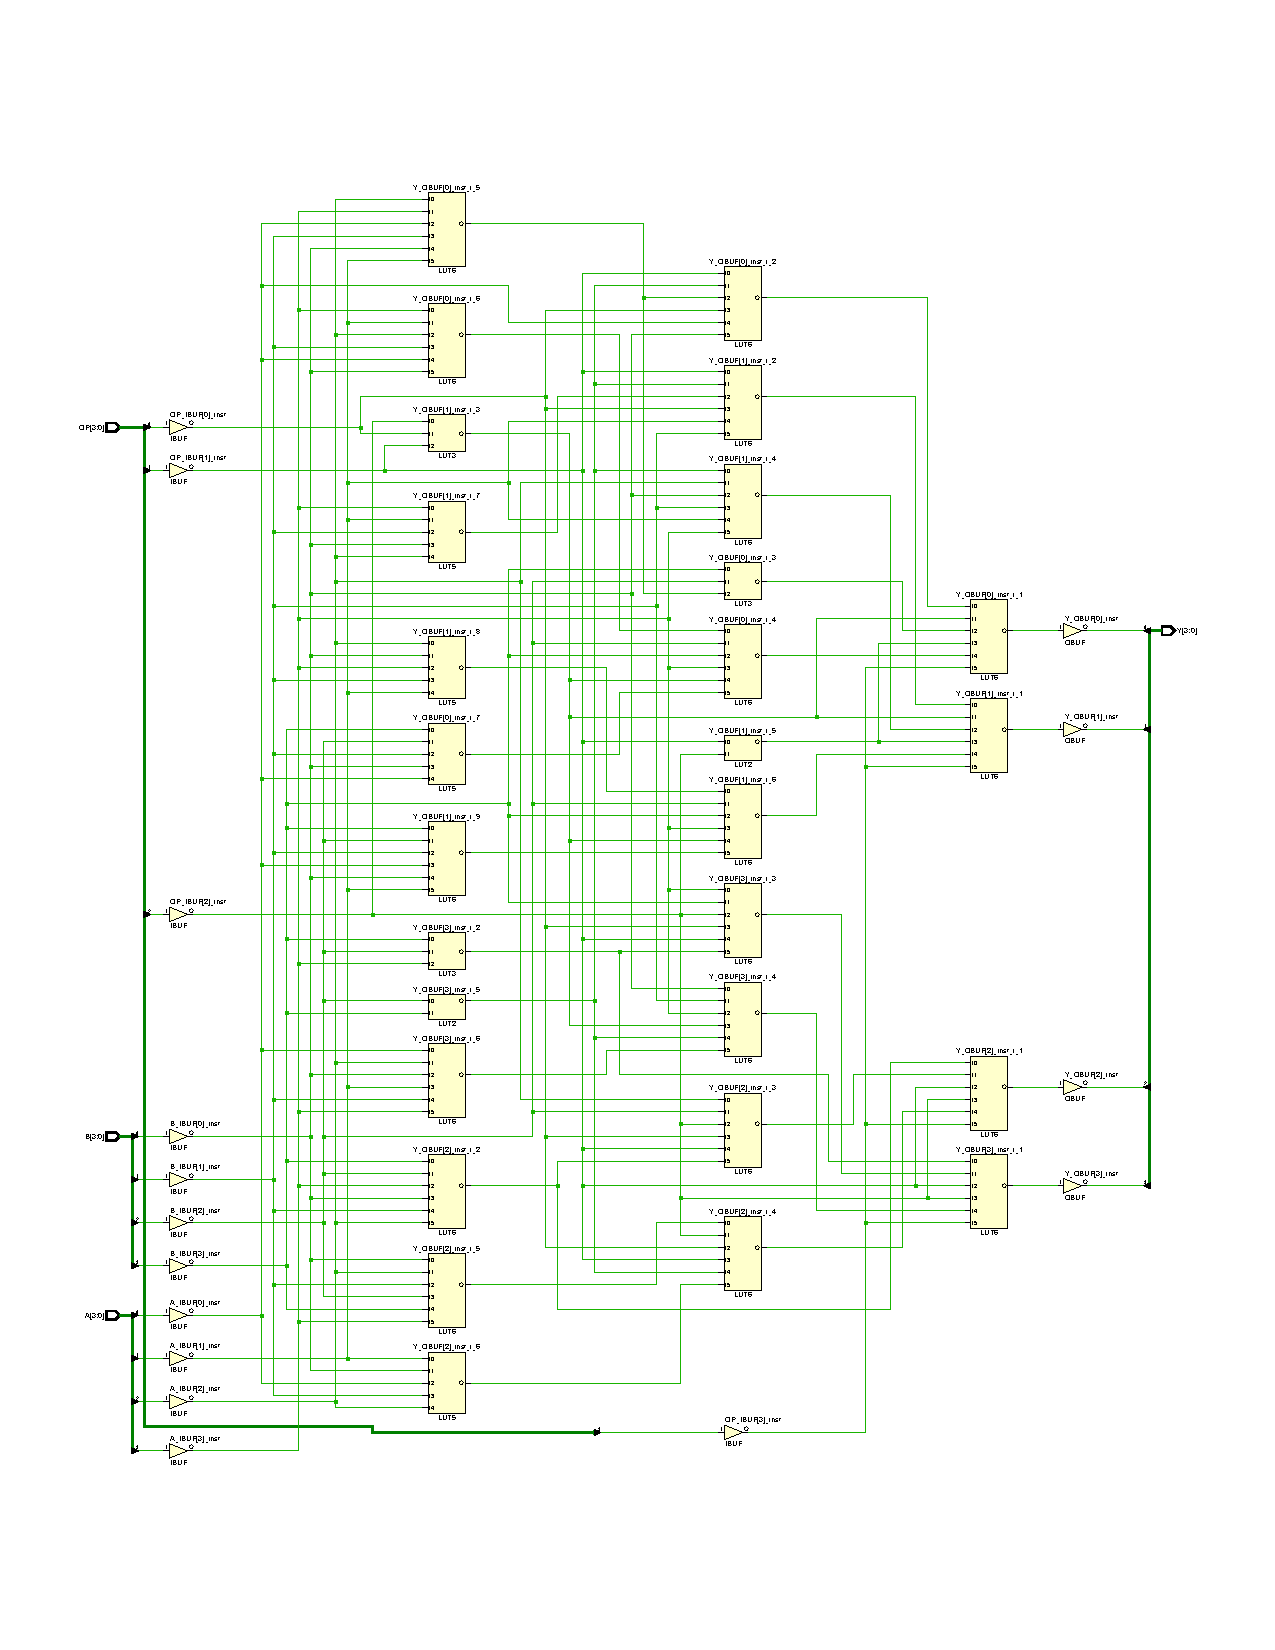
\includegraphics[width=\textwidth]{img/schematic}
        \caption{Synthesis Schematic}
        %! suppress = FigureNotReferenced
        \label{fig:demo3}
    \end{figure}
    \begin{figure}[h!]
        \centering
        \includegraphics[width=\textwidth]{img/implementation-timing}
        \caption{Post-Implementation Timing simulation}
        %! suppress = FigureNotReferenced
        \label{fig:demo4}
    \end{figure}
    \begin{figure}[h!]
        \centering
        \includegraphics[width=\textwidth]{img/utilization-report}
        \caption{Implementation Utilization Report}
        %! suppress = FigureNotReferenced
        \label{fig:demo5}
    \end{figure}
    \begin{figure}[h!]
        \centering
        \includegraphics
        {img/bitstream}
        \caption{Screen-capture of successful bitstream generation}
        %! suppress = FigureNotReferenced
        \label{fig:demo6}
    \end{figure}

\end{document}